Plovdiv's famous master chocolatier Bonny needs to cut a slab of chocolate with raisins. The chocolate is a rectangular block of identical square pieces. The pieces are aligned with the edges of the chocolate, and they are arranged in $N$ rows and $M$ columns, for a total of $N\cdot M$ pieces. Each piece has one or more raisins on it, and no raisins lie between or across pieces.

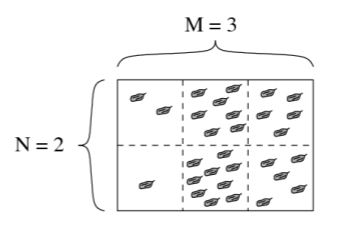
\includegraphics{raisins1.png}

Initially, the chocolate is one single, monolithic block. Bonny needs to cut it into smaller and smaller blocks until finally she has cut the chocolate down to its $N\cdot M$ individual pieces. As Bonny is very busy, she needs the help of her assistant, Sly Peter, to do the cutting. Peter only makes straight line, end-to-end cuts and he wants to be paid for every single cut he makes. Bonny has no money at hand, but she has plenty of raisins left over, so she offers to pay Peter in raisins. Sly Peter agrees to this arrangement, but under the following condition: every time he cuts a given block of chocolate into two smaller blocks, he has to be paid as many raisins as there are on the block he was given.

Bonny wants to pay Peter as little as possible. She knows how many raisins there are on each of the $N \cdot M$ pieces. She can choose the order in which she gives Peter any remaining blocks, and she can also tell Peter what cuts to make (horizontal or vertical) and where exactly to make them. Help Bonny decide how to cut the chocolate into individual pieces, so that she pays Sly Peter as few raisins as possible.

Write a program that, given the number of raisins on each of the individual pieces, determines the minimum number of raisins that Bonny will have to pay Sly Peter. 